\documentclass[11pt,a4paper]{ctexart}
\usepackage[margin=2.25cm]{geometry}
\usepackage{amsmath,amssymb,booktabs,array,longtable}
\usepackage{graphicx,float,xcolor}
\usepackage{hyperref}
\usepackage{listings}
\hypersetup{colorlinks=true,linkcolor=blue!55!black,urlcolor=blue!55!black}
\setlength{\parindent}{2em}
\setlength{\parskip}{0.35em}
\setlength{\emergencystretch}{2em}
\newcommand{\hpwl}{\operatorname{HPWL}}
\newcommand{\ov}{\operatorname{overflow}}
\newcommand{\code}[1]{\texttt{\detokenize{#1}}}

\title{精确非光滑 HPWL 的自适应 epsilon-active 求解\ 实现、消融与 ISPD2005 实验报告}
\author{HUAWEI\_EDA / DREAMPlace C++}
\date{2026 年 8 月 14 日}

\begin{document}
\maketitle

\begin{abstract}
本报告总结 DREAMPlace 风格 C++ 全局布局器中精确非光滑 HPWL 的 epsilon-active 实现，并报告八个 ISPD2005 数据集的实验结果。目标函数始终使用带 pin offset 的精确 HPWL，静电密度项通过逐网格电荷沉积和 Poisson 电场计算；没有用 weighted-average、log-sum-exp 或其他平滑 HPWL 替换评价目标。本文比较固定 epsilon、旧自适应控制器以及新设计的阶段感知 predictive 控制器，并额外测试按网 bbox span 截断 epsilon 的方法。a1/a2 筛选表明 predictive 控制器在 a2 略有收益，但在 a1 略有损失；硬 span cap 在两个数据集上均明显劣化。因此正式八组实验采用在前期进行窗口化 smart adaptive、进入 7\% overflow 可行带后冻结 epsilon 的稳健配置。a1--a4 和 bigblue1--3 的最终布局均通过内部合法性检查，最终合法 HPWL 相对论文 Table II 的 DREAMPlace V100 参考值平均高约 4.99\%（bigblue4 因 overflow 为 13.39\%，标记为未满足密度约束）。
\end{abstract}

\section{实验问题与可复现口径}

本轮实验回答两个问题：第一，能否用更精细的 epsilon 自适应方式改善固定 epsilon；第二，这种方法在八个 ISPD2005 设计上的精确 HPWL 与最终合法化结果如何。所有运行均从原始 Bookshelf 数据和中心高斯初始化开始，seed 为 1000，使用 Adam、静电密度、精确 HPWL 次梯度和 DREAMPlace 风格详细布局。默认调用方式没有改变，新控制器只有显式 CLI 开关才启用。

论文 Table II 的 DREAMPlace V100 HPWL 参考值为：adaptec1 73.22M、adaptec2 82.22M、adaptec3 193.72M、adaptec4 174.08M、bigblue1 89.38M、bigblue2 136.54M、bigblue3 303.90M、bigblue4 743.75M。论文表中的数值用于质量对比，不与本文的 GP overflow 或合法化时间混合解释。

\section{精确非光滑目标}

令 $p_i=(x_i+o_i^x,y_i+o_i^y)$ 为 cell $i$ 的 pin 坐标。全局布局目标写为
\begin{equation}
 F(x,y;\lambda)=H(x,y)+\lambda E_\rho(x,y),
\end{equation}
其中精确 HPWL 为
\begin{equation}
 H(x,y)=\sum_{e} w_e\left[\max_{i\in e}p_i^x-\min_{i\in e}p_i^x
 +\max_{i\in e}p_i^y-\min_{i\in e}p_i^y\right].
\end{equation}
该函数是分段线性的非光滑函数。对于每条网，普通次梯度只给当前极值 pin 施加方向；epsilon-active 方向在距离左右、上下极值不超过 epsilon 的 pin 集合内分配方向权重。若 $r$ 是当前 epsilon，权重为
\begin{equation}
 a(t)=\left(\max(0,1-t/r)\right)^q,
\end{equation}
并分别归一化左、右、下、上候选集合。这里 $q=4$。该构造只改变 trial direction，不改变 $H$ 的定义、接受判据或最终报告值。

\section{静电密度模型}

移动 cell、固定宏和 filler 以矩形电荷沉积到 $B_b$ 网格。沉积电荷为
\begin{equation}
 q_b=\sum_i r_i\,\operatorname{area}(R_i\cap B_b),
 \qquad r_i=\frac{w_i h_i}{\widetilde w_i\widetilde h_i},
\end{equation}
其中扩大的有效矩形避免单个小 cell 只落入一个网格，并由 $r_i$ 保持总电荷不变。电势通过离散 Poisson 方程求得，电场梯度反向收集到 cell 坐标。overflow 使用非 filler 的可移动面积归一化：
\begin{equation}
 \ov=\frac{\sum_b [q_b-\rho_t A_b]_+}{\sum_{i\in\mathrm{movable}} w_i h_i}.
\end{equation}
因此密度是逐网格建模、逐 cell 收集梯度，而不是对每个点单独施加孤立排斥力。

\section{epsilon 自适应策略}

\subsection{固定和第一代 smart 控制器}

固定模式保持初始 radius 不变。旧 adaptive 模式每 25 步根据 overflow 是否高于 7\%、是否低于 6.5\%、以及 HPWL 的单步变化修改全局 scale。第一代 smart 模式加入长度为 50 的历史窗口、overflow/HPWL 趋势、指数移动平均、deadband 和 log-step 上限。正式八组采用如下参数：
\begin{center}
\begin{tabular}{ll}
\toprule
参数 & 数值\\
\midrule
窗口 / 更新间隔 & 50 / 25\\
增益 / deadband & 0.5 / 0.0025\\
scale 下界 / 上界 & 0.70 / 1.10\\
最大 log-step & 0.03\\
可行带 & 6.5\%--7.0\%\\
\bottomrule
\end{tabular}
\end{center}

进入可行带后默认冻结 epsilon scale，以避免合法化敏感阶段的极值拓扑持续改变。该配置对应命令行开关 
\code{--adaptive-active-smart}，同时保持 \code{--adaptive-active-refinement} 未启用。

\subsection{第二代 predictive 控制器}

为探究更精细的策略，新增 opt-in 开关 \code{--adaptive-active-predictive}。它将控制过程分成三个阶段：
\begin{enumerate}
  \item 远离可行域时，比较 overflow 的实际下降与按剩余预算估计的期望下降，密度收敛滞后时扩大 epsilon；
  \item 接近 7\% 时，提高 overflow pressure 和 HPWL 趋势的权重，避免为密度继续牺牲线长；
  \item 进入 refinement 后使用更小的 log-step 上限，只允许小幅拓扑修正。
\end{enumerate}
其历史信号仍使用 EMA，因此 epsilon 的变化在 log 空间进行，且被 scale 上下界截断。该设计不引入平滑 HPWL。

另一个实验性选项 \code{--adaptive-active-span-cap} 将 epsilon 限制为每条网 bbox span 的某个比例。其动机是防止短网的同一 pin 同时落入左右 active 集合，但实验结果显示这种硬约束破坏了可布性，未纳入最终配置。

\section{自适应控制器的详细实现}

本节给出当前实现的逐步定义。需要区分两个独立的自适应量：\(\lambda_t\) 是静电密度项的权重，决定线长与密度在总方向中的相对比例；\(s_t\) 是 epsilon-active 半径的缩放因子，只改变精确 HPWL 次梯度的 trial direction。优化器实际使用
\[
 g_t=g_{\mathrm{HPWL}}^{\varepsilon_t}+\lambda_t g_{\mathrm{density}},\qquad
 \varepsilon_t=\varepsilon_{\mathrm{base}}s_t.
\]
因此，自适应控制并没有把 HPWL 替换成平滑函数。

\subsection{精确目标与 epsilon-active 方向}
对每条网，程序首先用真实 pin 坐标计算精确包围盒 HPWL。对于方向生成，除了当前最左、最右、最下和最上 pin 外，还考虑距离相应边界不超过 \(\varepsilon_t\) 的 pin。以左边界为例，候选 pin 的权重为
\[
 a_i^- = \left[\max\left(0,1-\frac{x_i-x_{\min}}{\varepsilon_t}\right)\right]^p,
 \qquad p=\texttt{active\_set\_power}.
\]
右、下、上边界分别使用对应距离，并对每一侧的权重单独归一化。于是每条网的 x 方向贡献是
\[
 g_{i,x}^{(e)}=w_e\left(\frac{a_i^+}{\sum_j a_j^+}-\frac{a_i^-}{\sum_j a_j^-}\right),
\]
y 方向完全类似。远离边界的 pin 权重为零，越接近极值的 pin 权重越大。\(p=4\) 使方向集中在近极值区域，同时比单一极值 pin 更不容易因极值切换而跳变。重要的是，CSV 中的 \(\hpwl\)、filter 接受条件和最终报告值都来自未修改的精确 HPWL。

\subsection{历史窗口和趋势信号}
程序每一步把精确 HPWL 和 overflow 分别写入两个历史队列，并保留最近 50 步。每 25 步更新一次半径；当窗口尚未达到至少半窗口长度时，不进行 smart 更新。更新时比较窗口后半段与前半段的代表值，得到
\[
 \Delta H=\frac{H_t-H_{t-k}}{\max(|H_{t-k}|,1)},\qquad
 \Delta O=O_t-O_{t-k}.
\]
\(\Delta H>0\) 表示线长上升，\(\Delta O>0\) 表示密度恶化。overflow 的约束优先级高于 HPWL：只有进入目标密度带后，HPWL 趋势才用于细调 epsilon。

\subsection{deadband、EMA 与对数半径更新}
目标 overflow 为 7\%，refinement 下界约为 6.5\%。在 7\% 附近设置 0.25 个百分点的 deadband，避免 6.99\%/7.01\% 的测量摆动导致方向频繁反转。由 overflow 压力、overflow 趋势和 HPWL 趋势组成的控制信号记为 \(q_t\)，再使用指数移动平均
\[
 s^{\mathrm{EMA}}_t=\rho s^{\mathrm{EMA}}_{t-1}+(1-\rho)q_t,
 \qquad \rho\approx0.70.
\]
最后在对数空间更新缩放因子：
\[
 s_{t+1}=s_t\exp(\delta_t),\qquad
 \delta_t=\operatorname{clip}(c\,s^{\mathrm{EMA}}_t,-\delta_{\max},\delta_{\max}).
\]
正式 smart 配置把缩放因子限制在 \([0.70,1.10]\)，单次最大对数步长为 0.03。乘法更新保证半径始终为正，并使增大和减小在相对尺度上对称。

\subsection{三个运行阶段}
在 overflow 明显高于目标时，控制器增加 epsilon，使更多近极值 pin 参与方向，同时由静电场承担主要密度恢复任务；当 overflow 接近 7\% 时，控制信号同时考虑密度压力和 HPWL 趋势；当布局进入 refinement/可行带后，基础半径从全局值过渡到较小的 refinement 半径，并冻结 smart scale 或仅允许极小更新，以免合法化敏感阶段的 active 集合继续大幅变化。adaptec1 的基础/精修半径为 125/50，adaptec2 为 165/65。

\subsection{lambda 的配合}
密度激活时，程序首先按 HPWL 与密度梯度的 L1 范数比初始化 \(\lambda\)。之后 lambda 控制器根据 overflow 轨迹和 HPWL 变化更新有效密度权重：overflow 超出目标带时提高密度压力，明显低于下界时降低压力，进入可行带后采用窄带控制。这个更新和 epsilon 控制相互独立：前者改变 \(g_{\mathrm{density}}\) 的系数，后者改变 \(g_{\mathrm{HPWL}}^{\varepsilon}\) 的分布。两者共同作用，但都不改变精确 HPWL 的评价函数。

\subsection{为什么不直接使用单步规则}
单步规则会对极值 pin 切换、静电网格离散误差和 Adam 历史动量都过于敏感。50 步窗口提供时间尺度上的趋势，deadband 消除目标附近的抖动，EMA 抑制异常点，对数步长和上下界限制最坏情况下的方向变化。实验中硬性按 bbox span 截断 epsilon 会使 a1 的 GP HPWL 增加约 8.5M，因此没有纳入正式配置。

\section{a1/a2 筛选实验}

所有筛选使用 800 步、无 GP 合法 checkpoint 抽样，以隔离优化本身的时间和数值。

\begin{table}[H]
\centering
\small
\caption{a1/a2 的 epsilon 策略筛选。HPWL 单位为 M；legal 为最终内部详细合法化结果。}
\begin{tabular}{lrrrrrrr}
\toprule
策略 & 迭代次数 & a1 GP & a1 legal & a2 GP & a2 legal & 说明\\
\midrule
固定 epsilon（历史） & 800 & 72.669 & 76.996 & 82.715 & 83.922 & 基线\\
smart（正式配置） & 800 & 72.695 & 76.621 & 80.003 & 82.375 & 八组采用\\
predictive（温和参数） & 800 & 72.650 & 76.732 & 79.938 & 82.331 & a2 略有收益\\
predictive + span 0.50 & 800 & 81.308 & 86.776 & -- & -- & 明显失败\\
predictive + span 0.35 & 800 & 81.158 & 86.680 & -- & -- & 明显失败\\
\bottomrule
\end{tabular}
\end{table}

predictive 的结论是数据集依赖的：a2 合法 HPWL 改善约 0.044M，但 a1 劣化约 0.111M。硬 span cap 在 a1 的 GP 就增加约 8.5M，说明 active 集合的适度重叠可能提供了有用的分布式方向，不能用简单几何截断代替时间控制器。因此正式八组选择跨数据集更稳健的 smart 配置。

\begin{table}[H]
\centering
\small
\caption{固定 epsilon 与 smart adaptive 的直接对比。两种方法使用相同的数据集和迭代预算；HPWL 单位为 M，改善值定义为固定 epsilon 合法 HPWL 减去 smart adaptive 合法 HPWL。固定 epsilon 结果来自六设计非自适应正式实验。}
\begin{tabular}{lrrrrrr}
\toprule
设计/迭代 & 固定 GP & 固定 legal & smart GP & smart legal & 改善(M) & 改善(\%)\\
\midrule
adaptec1/1400 & 72.671 & 76.641 & 72.695 & 76.621 & 0.020 & 0.03\\
adaptec2/1600 & 82.715 & 83.922 & 80.003 & 82.375 & 1.547 & 1.84\\
adaptec3/1600 & 189.353 & 200.002 & 189.520 & 200.042 & -0.040 & -0.02\\
adaptec4/1600 & 175.989 & 182.683 & 176.185 & 183.137 & -0.454 & -0.25\\
bigblue1/1600 & 87.636 & 89.810 & 87.617 & 89.759 & 0.051 & 0.06\\
bigblue2/1600 & 136.791 & 143.495 & 136.708 & 143.328 & 0.167 & 0.12\\
\bottomrule
\end{tabular}
\end{table}

该六设计对比表明，自适应 epsilon 的收益具有数据集依赖性。adaptec2 的合法 HPWL 改善最大，达到 1.547M（1.84\%）；adaptec1、bigblue1 和 bigblue2 也有小幅改善。adaptec3 和 adaptec4 的 smart 结果略差，说明当前单一的跨数据集窗口和缩放边界还不能保证所有设计都受益。另需注意，adaptec1 的 smart GP 比固定配置高 0.024M，但合法化后仍改善 0.020M，说明自适应策略的价值不只体现在连续 GP 阶段的瞬时 HPWL，也体现在对后续 row/segment 合法化的适配性。

\begin{table}[H]
\centering
\small
\caption{六个设计的 epsilon 半径设置。非自适应实验关闭 adaptive scale，因而 scale 始终为 1；箭头表示进入 refinement 后从全局半径过渡到精修半径。smart adaptive 使用相同的基础半径，但允许 scale 在给定范围内缓慢变化。}
\begin{tabular}{lrrrr}
\toprule
设计 & 非自适应全局半径 & 非自适应精修半径 & smart 全局/精修半径 & smart scale 范围\\
\midrule
adaptec1 & 125 & 50 & $125\rightarrow50$ & 0.70--1.10\\
adaptec2 & 165 & 165 & $165\rightarrow65$ & 0.70--1.10\\
adaptec3 & 265 & 105 & $265\rightarrow105$ & 0.70--1.10\\
adaptec4 & 265 & 105 & $265\rightarrow105$ & 0.70--1.10\\
bigblue1 & 125 & 50 & $125\rightarrow50$ & 0.70--1.10\\
bigblue2 & 212 & 85 & $212\rightarrow85$ & 0.70--1.10\\
\bottomrule
\end{tabular}
\end{table}

因此，表中的“非自适应”不是指所有迭代始终使用同一个绝对半径，而是指不根据 HPWL/overflow 历史改变半径 scale。非自适应路径仍可能在进入 refinement 时执行预先设定的半径过渡；smart adaptive 则在此基础上叠加窗口化控制，并在可行带附近冻结或限制 scale 的变化。

\section{八个 ISPD2005 数据集结果}

\begin{table}[H]
\centering
\scriptsize
\caption{正式 smart adaptive 结果。GP 是精确非光滑全局布局；legal 是完整内部合法化和详细布局后 HPWL。}
\begin{tabular}{lrrrrrrrrr}
\toprule
设计 & 迭代次数 & GP HPWL & GP overflow & legal HPWL & 论文参考 & 劣化 & legal & 状态\\
\midrule
adaptec1 & 1400 & 72.695 & 6.994\% & 76.621 & 73.22 & 4.64\% & yes & pass\\
adaptec2 & 1600 & 80.003 & 6.989\% & 82.375 & 82.22 & 0.19\% & yes & pass\\
adaptec3 & 1600 & 189.520 & 6.976\% & 200.042 & 193.72 & 3.26\% & yes & pass\\
adaptec4 & 1600 & 176.185 & 6.990\% & 183.137 & 174.08 & 5.20\% & yes & pass\\
bigblue1 & 1600 & 87.617 & 6.999\% & 89.759 & 89.38 & 0.42\% & yes & pass\\
bigblue2 & 1600 & 136.708 & 6.976\% & 143.328 & 136.54 & 4.97\% & yes & pass\\
bigblue3 & 2400 & 310.461 & 6.980\% & 342.040 & 303.90 & 12.55\% & yes & pass\\
bigblue4 & 1600 & 802.418 & 13.393\% & 808.137 & 743.75 & 8.66\% & yes & density fail\\
\bottomrule
\end{tabular}
\end{table}

除 bigblue4 外，正式 GP 均进入 7\% overflow 带。最终合法 HPWL 相对论文参考的逐设计平均劣化为 4.99\%；若排除未满足密度约束的 bigblue4，前七个设计的算术平均劣化约为 4.46\%，总 HPWL 比值约为 1.061。bigblue4 的最终合法性为真，但 overflow 仍为 13.393\%，所以不能把它作为满足同一密度约束的公平质量比较。

\begin{figure}[H]
  \centering
  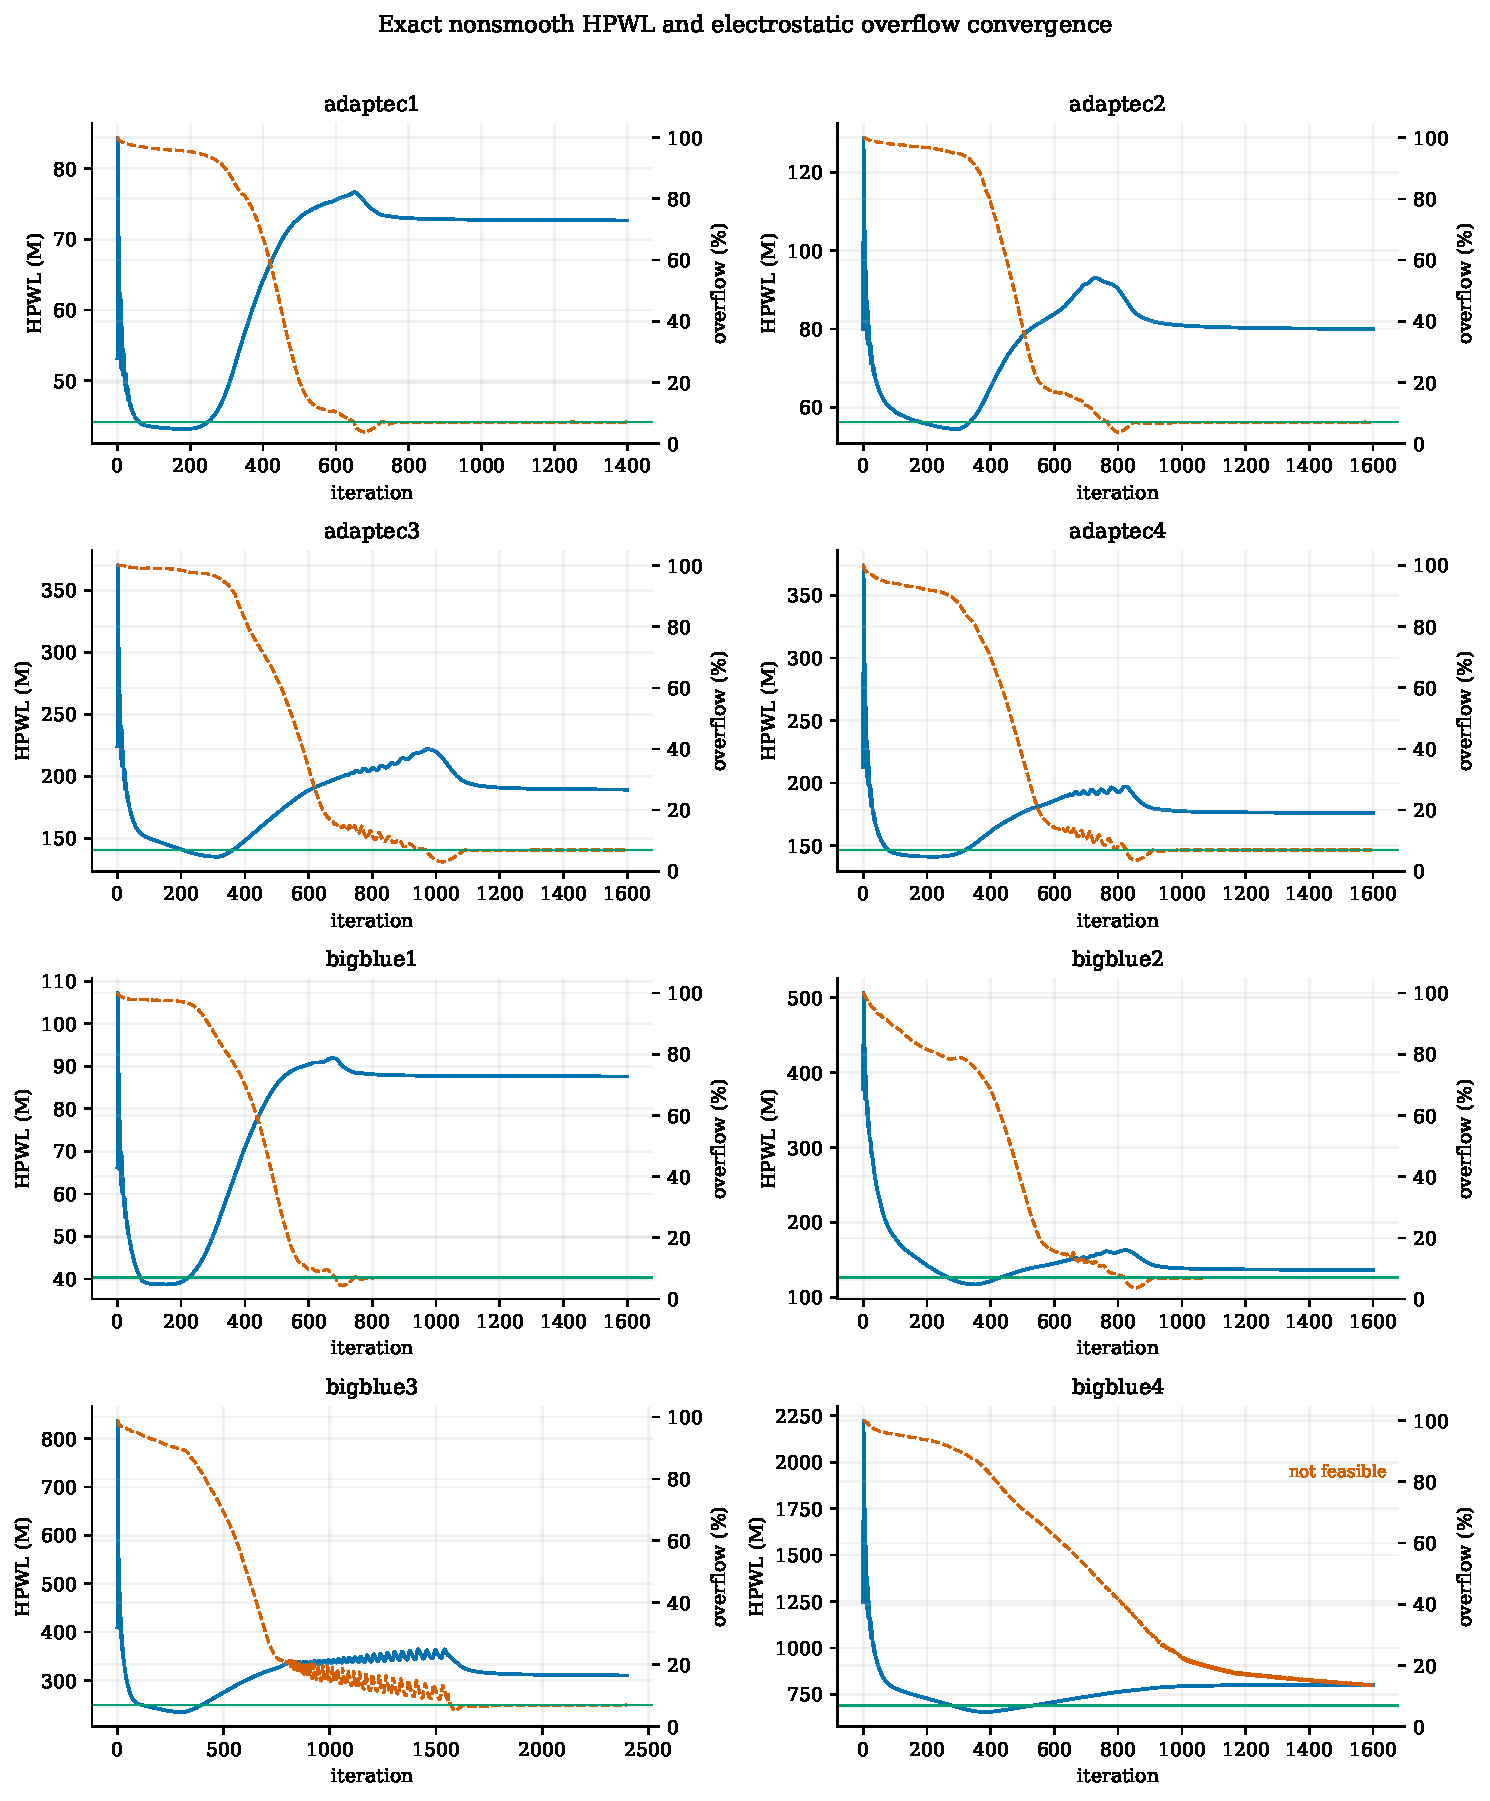
\includegraphics[width=0.98\textwidth]{figures/adaptive_epsilon_convergence.pdf}
  \caption{八个数据集的精确 GP HPWL 和静电 overflow 收敛曲线。蓝线为精确 HPWL，橙色虚线为 overflow，绿色窄带为 6.5\%--7.0\%。bigblue3 使用正式运行前已达到可行带的原始曲线，随后使用多行高合法化重试；bigblue4 明确标记为未达到密度约束。}
\end{figure}

\begin{figure}[H]
  \centering
  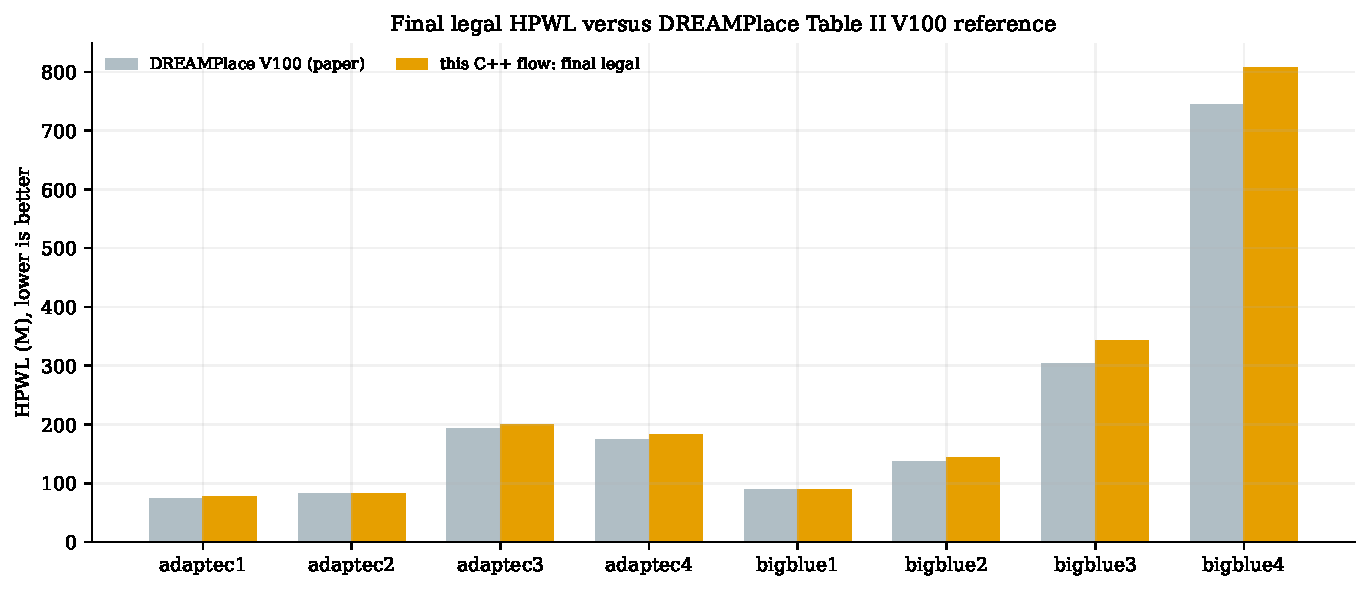
\includegraphics[width=0.95\textwidth]{figures/adaptive_epsilon_vs_dreamplace.pdf}
  \caption{最终内部合法 HPWL 与 DREAMPlace 论文 Table II 的 V100 HPWL 参考值。}
\end{figure}

\section{合法化流程与合法性检查}

全局布局阶段不把“任何移动 cell 不得进入固定宏”作为硬约束，而是在后处理阶段逐步完成合法化。当前流程为：
\begin{enumerate}
  \item 从 GP 坐标建立 obstacle-aware row segments；
  \item locality-first Greedy 将 cell 放入候选 row/segment，并按站点对齐；
  \item 失败时恢复 GP 连续坐标，执行 width-first 和容量感知 best-fit 回退；
  \item Abacus 对每个 row segment 做局部二次代价压缩；
  \item DREAMPlace 风格 K-Reorder、global swap、independent-set matching 和 cell insertion 进行离散 HPWL 改善；
  \item 对多行高 cell，检查连续 row 的公共可用区间并一次性预留其跨行 footprint；
  \item 最后执行站点取整、局部 row re-legalization 和完整检查。
\end{enumerate}

内部检查逐 cell、逐覆盖 row 验证边界、站点对齐、移动 cell 相互重叠和固定宏重叠。八个正式输出的\code{summary.txt} 均为 \code{internal_legal=true}，且 boundary、alignment、overlap 三类错误均为 0。当前 Windows 环境没有可用 Perl，因此未能执行用户提供的官方 \code{legal2.pl}；报告中的“合法”是内部几何检查，不冒充官方脚本结果。

\section{性能与实现注意事项}

正式八组开启 \code{--legal-checkpoints}，因此总 wall time 包含周期性快速合法化，不能直接与仅 GP 的论文 GPU 时间比较。a1/a2 的无 checkpoint 800 步筛选中，单次 GP 约 22--23 秒；开启详细 checkpoint 后，a1/a2 正式运行分别约 292 秒和 494 秒。性能瓶颈来自高分辨率 CPU 静电网格、矩形电荷沉积、逐 cell 电场回收和合法化抽样，而不是 epsilon 公式本身。论文 DREAMPlace 使用 GPU DCT/IDCT、合并的 density forward/backward kernel 和高度并行的详细布局，因此不能仅凭 C++ CPU 迭代次数推断同量级运行时间。

\section{失败尝试与改进建议}

本轮实验没有把失败候选隐藏起来。predictive 控制器在 a2 有小幅收益但在 a1 变差，说明单一跨设计参数仍不足。span cap 的失败说明短网 active 集合重叠并非纯噪声。bigblue4 的续跑还揭示了一个工程问题：当前 \code{global.pl} 只保存 movable 坐标，重新运行时 filler 会重新随机初始化，不能直接作为保留完整静电状态的 continuation checkpoint；因此该续跑被停止，未计入正式结果。

后续最值得做的改进有三项。第一，保存和恢复 filler 坐标、density grid 和 Adam moments，才能进行真正连续的 bigblue4 续跑。第二，把 epsilon 控制器扩展为按 cell density sensitivity 分组的多时间尺度控制，而不是按 bbox span 硬截断。第三，在进入 7\% 后用稀疏 quick-legal HPWL 作为 checkpoint 选择信号，并保持默认低频率，避免把合法化开销放进每一步优化。

\section{结论}

当前实现已经形成一条可复现的精确非光滑 HPWL 流程：epsilon-active 只用于生成非光滑 trial direction，静电场负责网格密度恢复，Adam 与窄带 lambda 控制负责连续优化，Greedy/Abacus/DREAMPlace-style detailed placement 负责离散合法化。smart adaptive 是目前最稳健的八组默认策略；predictive 控制器和 span cap 提供了明确的消融结论，但暂不足以替代正式配置。a1、a2、a3、a4、bigblue1、bigblue2、bigblue3 均同时达到内部合法和约 7\% GP overflow，bigblue4 则需要保存完整 filler 状态和更强的高分辨率密度求解才能成为公平的 baseline 对比点。

\end{document}
